\subsection{Report binding and challenge--response verification}
The four-valued rule defines the evidence--policy relationship, but a geometric proof by itself cannot prevent the proof from being carried over to a different report or task. The prototype therefore uses the expiring challenge--response flow in Figure~\ref{fig:sequence}.

An administrator configures the task, verifying key, spacetime policy, threshold, and ordered issuer roster. The gateway retains a trusted snapshot of these settings and rejects repeated keys or trust-domain labels. It then generates a random 256-bit challenge $\nu$ using a trusted application clock and assigns an expiry time $e$. The vehicle and issuers derive a shared context:
\begin{equation}\label{eq:context}
c=\operatorname{OS2IP}\!\left(\operatorname{SHA256}\!\left(
\operatorname{Encode}(v,T,\nu,e,\operatorname{SHA256}(R))
\right)\right)\bmod q.
\end{equation}
Here $v$ is the protocol version, $T$ is the configured task, $R$ is the report's original byte sequence, $q$ is the BN254 scalar-field modulus, and $\operatorname{OS2IP}$ maps a byte sequence to an integer. Context $c$ binds the signed evidence and proof statement to a specified report and challenge. It neither encrypts the report nor hides its contents.

The implementation uses a Go JSON structure with fixed field order and no map fields. The report's SHA-256 digest is written as lowercase hexadecimal, and the issuer public-key byte arrays follow Go JSON's Base64 encoding. This defines deterministic bytes for the present prototype, not a standardized cross-language canonicalization. Implementations in other languages must reproduce the exact serialized bytes or agree upon a separately specified canonical format.

Each issuer signs a message digest containing $c$ and its measured interval. After collecting all signatures required by the roster, the vehicle applies Section~3.2's decision rule and constructs a zero-knowledge proof $\pi$ with interval endpoints and signatures as private witness data. The gateway checks the challenge's existence and validity period, reconstructs the public inputs from its trusted task snapshot and received report bytes, and checks the proof together with its decision code. It accepts only a proven Valid decision.

A successful verification atomically marks the nonce as used inside the current gateway instance. In the concurrent test with eight copies of one valid request, only one is accepted. Failed proof verification leaves an unexpired challenge available for legitimate retries; nevertheless, repeated invalid submissions can exhaust verification resources, so rate limiting is needed in deployment. The prototype neither persists nonce state across restarts nor implements distributed atomicity across gateway replicas. New nonces also do not, on their own, prevent resubmission of identical business reports.
\begin{figure}[htbp]\centering
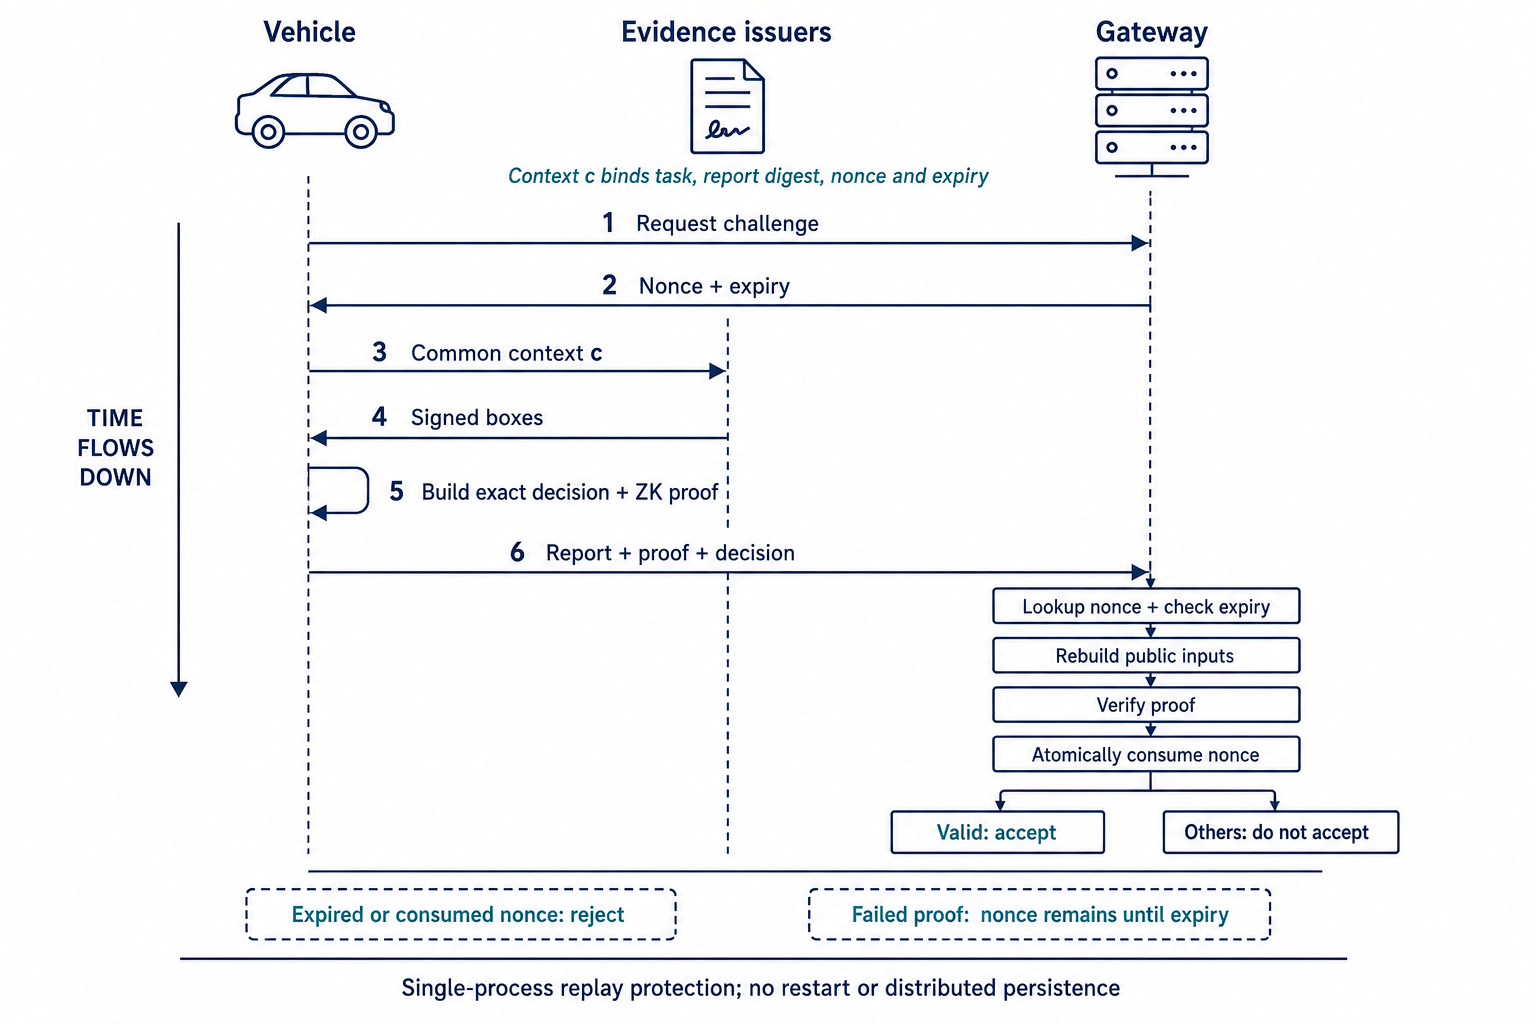
\includegraphics[width=\linewidth]{../figures/protocol_sequence.png}
\caption{Report-bound challenge and verification flow. After successful proof verification the gateway atomically marks the nonce as used within its current instance; failed attempts leave the challenge available for retries until expiry. Network transport details are omitted.}\label{fig:sequence}
\end{figure}
